\documentclass{beamer}
\usetheme{default}
\usepackage{amsmath}
\usepackage{xcolor} % before tikz or tkz-euclide if necessary
\usepackage{tkz-euclide} % no need to load TikZ
\usepackage{multirow}

\usepackage[
backend=biber,
style=authoryear-icomp,
sortlocale=de_DE,
natbib=true,
url=false, 
doi=true,
eprint=false
]{biblatex}
\addbibresource{../../Bibliography/main_ML.bib}

\titlegraphic{
\includegraphics[width=2cm]{../../Figures/UAMS_RGB.png}
}

\title{Statistical Machine Learning\\ Lecture 1 \\ Statistical Setup}
\author{Horacio G\'omez-Acevedo\\ Department of Biomedical Informatics}
\begin{document}
\begin{frame}[plain]
    \maketitle
\end{frame}
\begin{frame}{Introduction}
	
	We will fill the technical gaps of the Chapter 2 from G\'eron's book. 
	
	The objective of that chapter is:  Your model should learn from the provided data and be able to predict the median housing price in any district, given all the other metrics. 
	
	Rough methodology:
	\begin{itemize}
		\item It is a supervised learning model 
		\item Regression task 
		\item There is no continuous data flow 
		\item Sample size is small enough to handle it locally, thus a {\bf plain batch training} is appropriate.
	\end{itemize}
	
\end{frame}

\begin{frame}{Formal Setup}
	The book uses the following description for the data setup. Note however that at this point, the data is not a matrix yet (entries of features are not necessarily real numbers), thus we will call it a {\bf data frame}.
\begin{equation*}
	\mathbf{X}=
\bordermatrix{~ & feature\ 1 & feature\ 2 & \cdots & feature\ n   \cr
	(\mathbf{x}^{(1)} )^t& x_{11} & x_{12} & \cdots & x_{1n}   \cr
	(\mathbf{x}^{(2)} )^t& x_{11} & x_{12} & \cdots & x_{2n}   \cr
			 & \vdots & \vdots & \ddots & \vdots &  \cr
	(\mathbf{x}^{(m)} )^t & x_{m1} & x_{m2} & \cdots & x_{mn}  \cr} 
	\end{equation*}
and the response variable as 
$$
\mathbf{Y}=  (y^1, y^2, \ldots , y^m)
$$


\end{frame}

\begin{frame}{Matrix representation}
	Once we have transformed our data frame into a real matrix $\mathbf{X}$ of size $m \times n$ ($m$ observations and $n$ numerical features or predictors), the regression problem reduces to the representation of the response vector $Y$ as a function (or hypothesis) $h$ as follows
	\begin{equation}
		Y= h(X)+ \varepsilon
	\end{equation}
where $\varepsilon$ is a random error term. 

{\bf Important points}

\begin{itemize}
	\item We do not know $h$ beforehand
	\item It is customary to consider that the error rate averages zero
	\item Prediction of $Y$ can be done by using
	\begin{equation*}
		\hat{Y}= \hat{h} (X)
	\end{equation*}
 where  $\hat{h}$ is the estimate for $h$, and $\hat{Y}$ represents the resulting prediction of $Y$.
\end{itemize}
	
\end{frame}

\begin{frame}{Performance measure}
	
In a typical statistical framework, we measure the quality of fit to asses how well our approximation "fits" the data. Residuals are normally used to determine how well our model fits the data by the so-called  {\bf Residual Standard Error} (RSE)
\begin{equation}
	RSE= \sqrt{\frac{1}{m-2} \sum_{i=1}^m (h(x^{(i)})-y^{(i)})^2}
\end{equation}
A small variation is this formula is called {\bf Root Mean Squared Error (RMSE)}
\begin{equation}
	RMSE= \sqrt{\frac{1}{m} \sum_{i=1}^m (h(x^{(i)})-y^{(i)})^2}
\end{equation}
RMSE or (MSE) are normally used to determine the "performance" of our models.
\end{frame}
\begin{frame}{Norms in $\mathbb{R}^n$}
	So far the model has used the norm (distance) between two vectors as the Euclidean norm ($\ell_2$) as
	\begin{equation*}
		\ell_2 \colon \| \mathbf{x} \|_{2}= \sqrt{ \sum_{i=1}^n x_i^2}
	\end{equation*}
There are more "norms" (distances) that we can use
\begin{equation*}
		\begin{split}
				\ell_1 &\colon \| \mathbf{x} \|_{1}=  \sum_{i=1}^n |x_i|\\
	\ell_p &\colon \| \mathbf{x} \|_{p}= \sqrt[p]{ \sum_{i=1}^n |x_i|^p}	\\
	\ell_\infty&\colon \| x\|_\infty = \max_{i=1,\ldots,n} |x_i|	
		\end{split}
\end{equation*}
\end{frame}

\begin{frame}{Norms in the plane }
	When we consider a distance (norm), we want to visualize points that are close to zero up to a distance $\rho$. These sets are called (closed) balls of radius $\rho$. 
\begin{figure}
	\centering
	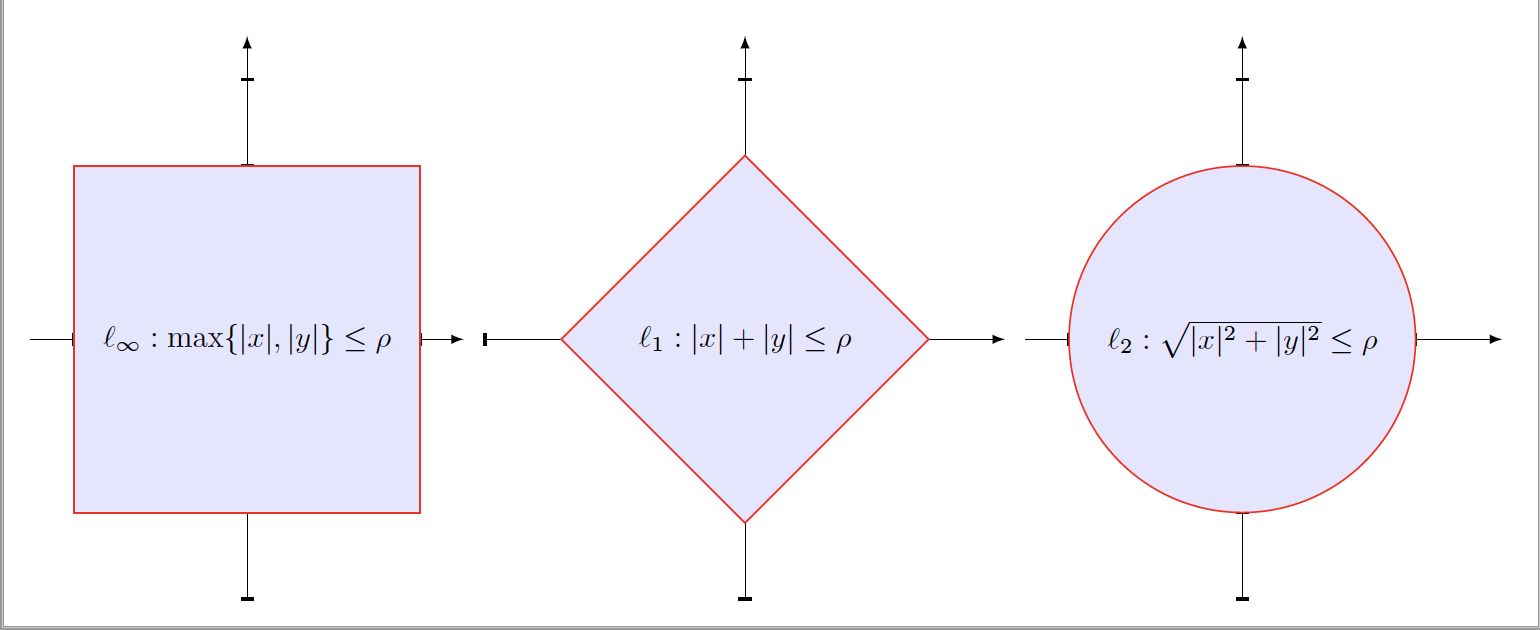
\includegraphics[scale=0.35]{../../Figures/fig_lp_metrics.png}
\end{figure}
These shapes will be important when we use Lasso techniques.

\end{frame}

\begin{frame}{Creating a Test Dataset}
	
	After we downloaded the data and roughly observed their distribution (through histograms). We proceed with a very important steps in any machine learning algorithm.
	
	\begin{itemize}
		\item Create a training set (typically around 80\% of the whole dataset)
		\item The rest will be the test set.
		\item {\bf Never ever peak at the test set}. This is a good scientific practice. 
		\item Use stratification and randomization to get proper representatives of the sample structure.
	\end{itemize} 
\end{frame}

\begin{frame}{Expectation}
	
	{\bf Informally: }
	Suppose $W$ represents the outcome of an experiment (say tossing a die). The {\bf expectation of W} (denoted by $E(W)$) can be perceived as the arithmetic mean of the outcome of $W$ when repeating the experiment many times. 
	
	{\bf Formally: }
	If $W$ is a random variable, then
	\begin{itemize}
		\item $W$ is discrete
		\begin{equation*}
			E(W)= \sum_{\alpha} \alpha P(W=\alpha)
		\end{equation*}
	\item $W$ is continuous with probability density function $f(w)$
	\begin{equation*}
		E(W)= \int_{-\infty}^\infty s f(s) ds
	\end{equation*}
	\end{itemize}
\end{frame}

\begin{frame}{Example}
	Suppose $W$ is the outcome when we roll a die. What is $E(W)$?
	
{\it Solution.} Since the die is fair $p(W=1)= p(W=2)= \cdots=p(W=6)=\frac 16$	
\begin{equation*}
\begin{split}
	E(W)&= 1 \left (\frac 16 \right) + 2 \left( \frac 16\right)+ 3 \left( \frac 16 \right) + 4 \left(\frac 16\right)+ 5 \left( \frac 16 \right) + 6 \left( \frac 16 \right)\\
	&= \frac 72
\end{split}
\end{equation*}

{\bf Note.} Not all random variables have expected value. For instance if $W$ is Cauchy distributed with parameters $\alpha =0$ and $\beta =1$. 
\end{frame}

\begin{frame}{Expectation properties}

Let's suppose that $W$ and $Z$ have expectations	
	\begin{itemize}
		\item Linearity: $E(aW+bZ)=a E(W)+b E(Z)$ where $a,b \in \mathbb{R}$
		\item Independence condition: If $W$ and $Z$ are (statistically) independent $E(WZ)= E(W)E(Z)$.
	\end{itemize}
If the expectation of $E(W^2)$ exists, we define the {\bf variance} of $W$ as
\begin{equation*}
\textrm{Var}(W)= E(W^2)-E(W)^2
\end{equation*}
If the variance of $Z$ also exists, we define the {\bf covariance} of $W$ and $Z$ as
\begin{equation*}
	\textrm{Cov}(W,Z)= E(WZ) - E(W)E(Z)
\end{equation*}

\end{frame}

\begin{frame}{Variance and Covariance Properties}
	\begin{itemize}
		\item Since $\textrm{Var}(W) \ge 0$, we define the {\bf standard deviation} of $W$ as $\sigma(W)=\sqrt{\textrm{Var}(W)}$
		\item $\textrm{Var}(W+Z)= \textrm{Var}(W)+ \textrm{Var}(Z)$
		\item $\textrm{Var}(aW)= a^2 \textrm{Var}(W)$ for $a \in \mathbb{R}$
		\item If $W$ and $Z$ are (statistically) independent $\textrm{Cov}(W,Z)= 0$.
		\item $\textrm{Cov}(W+a,Z+b)= \textrm{Cov}(W,Z)$
	\end{itemize}
	
	If $W$ is a random variable with existing variance, the {\bf standardize form of } $W$ is the variable $\tilde{W}$ defined by 
	\begin{equation*}
		\tilde{W}= \frac{W - E(W)}{\sigma(W)}
	\end{equation*}
It can be shown that
\begin{equation*}
	E(\tilde{W})=0 \quad \textrm{and} \quad \textrm{Var}(\tilde{W})= 1
\end{equation*}
\end{frame}

\begin{frame}{Variance Covariance Matrix}
	Let's go back and consider $X$ as a matrix of size $m \times p$.
	Thus, $X=(X_1, X_2, \ldots, X_p)$ where each $X_i$ is a column vector. We can calculate the so-called Variance-Covariance matrix
	\begin{equation*}
		\begin{pmatrix}
			\textrm{Var}(X_1) & \textrm{Cov}(X_1,X_2) & \cdots & \textrm{Cov}(X_1,X_p) \\
			\textrm{Cov}(X_2,X_1) & \textrm{Var}(X_2) & \cdots & \textrm{Cov}(X_2,X_n) \\
			\vdots & \vdots & \ddots & \vdots\\
			\textrm{Cov}(X_p,X_1) & \textrm{Cov}(X_p,X_2) & \cdots & \textrm{Var}(X_p)
		\end{pmatrix}
	\end{equation*}

\begin{itemize}
	\item All entries in the matrix are {\bf estimates} of the true variance and covariance.
	\item The matrix is symmetric.
\end{itemize} 
\end{frame}

\begin{frame}{Pearson's Correlation Coefficient}
If $W$ and $Z$ are random variables with existing variance and if neither $\sigma(W)$ nor $\sigma(Z)$ are zero. The {\bf Pearson's correlation coefficient} $\rho$ between $W$ and $Z$ is defined as

\begin{equation*}
	\rho(W,Z)= \frac{\textrm{Cov}(W,Z)}{\sigma(W)\sigma(Z)}
\end{equation*}
If $W$ and $Z$ are random variables with existing correlation coefficient, then
\begin{equation*}
	-1 \le \rho(W,Z) \le 1
\end{equation*}
When $\rho(W,Z)$ we say that $W$ and $Z$ are positively correlated. And similarly when $\rho(W,Z) < 0$ we called the variables negatively correlated. 



\end{frame}

\begin{frame}{Correlations (Important Notes)}

\begin{itemize}
	\item Even when the variables $W$ and $Z$ are perfectly correlated (i.e., $\rho(W,Z)= \pm 1$) this statement does not mean anything about {\it causation}. 
	\item Neither is true that $\rho(W,Z)=0$ implies (statistical) independence of $W$ and $Z$.
	\item Correlations do not catch non-linear relationships. 
\end{itemize}
\begin{figure}
\centering
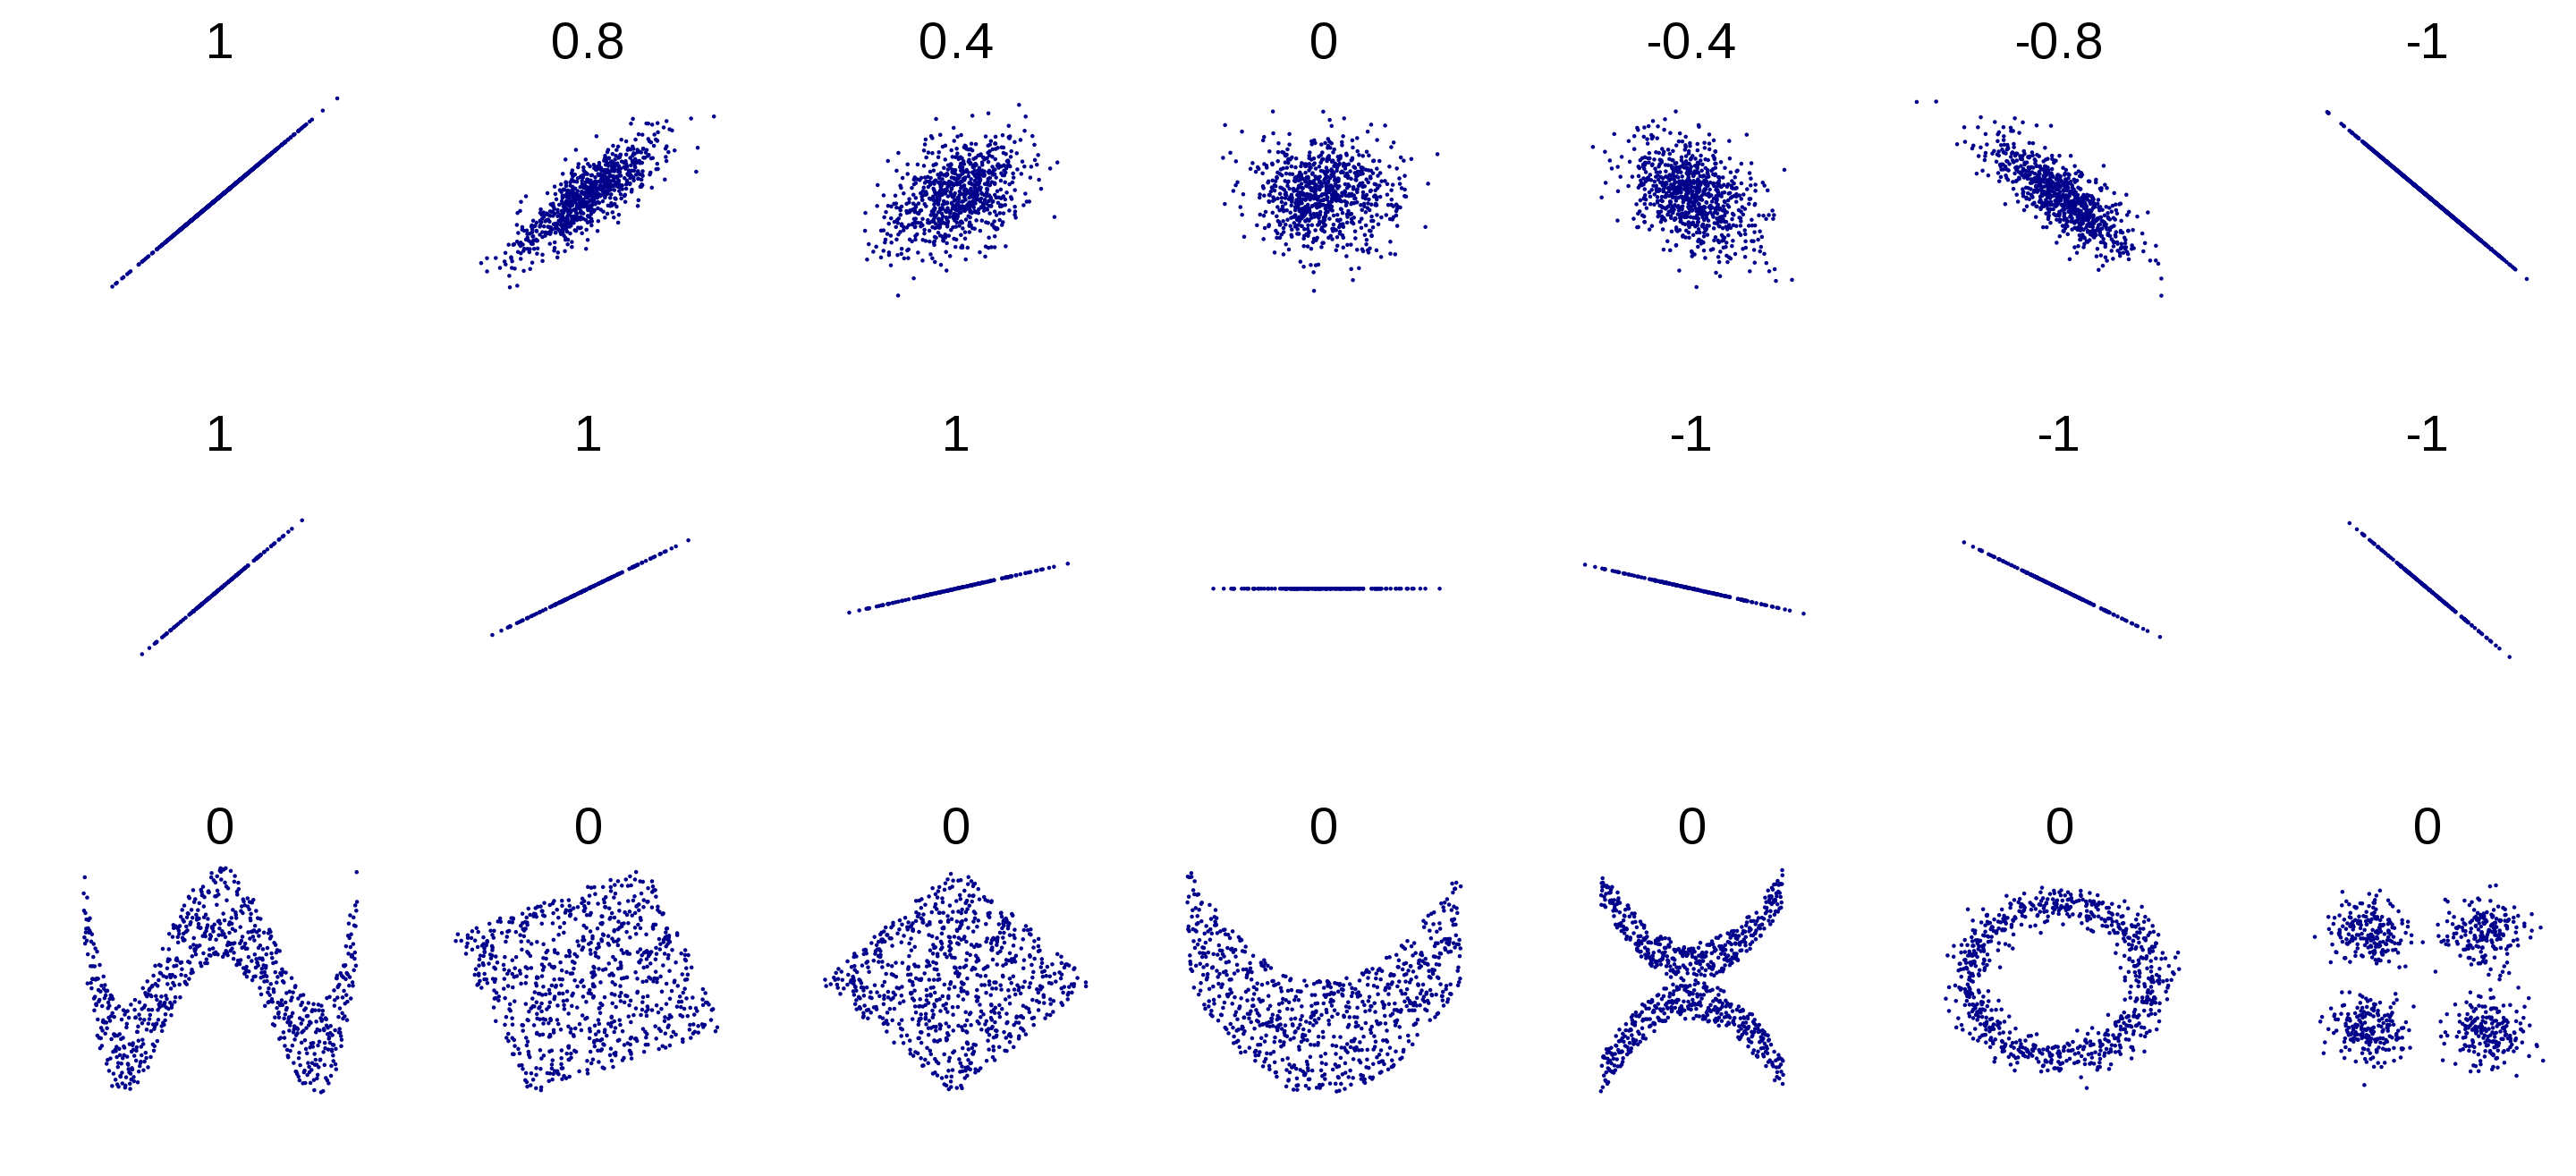
\includegraphics[scale=0.1]{../../Figures/fig_correlations.png}
\end{figure}
\end{frame}

\begin{frame}{The problem of collinearity}
	
	Highly correlated attributes (features) represent a problem for finding an appropriate model for our data.
	
	The simplest way to do it (even not the best) is to select one of the highly correlated variable. 
	
	There are more robust techniques to deal with collinearity (at least from the linear regression setup)
	\begin{itemize}
		\item Regression on principal components
		\item Ridge regression 
	\end{itemize}

\end{frame}

\begin{frame}{Data Imputation}
	When we face incomplete information or missing data our statistical tools do not normally work (or work poorly). One remedy is  "guess" the best possible value is a process called {\bf Data Imputation}.
	
	Let's consider a simple multilinear regression model 
	\begin{equation*}
		Y= \beta_0 + \beta_1 X_1 + \beta_2 X_2 + \cdots+ \beta_p X_p + \varepsilon 
	\end{equation*}
	
	One simple method is the {\it case-wise deletion}, which means that a if we have a missing value in any of our variables we drop that data point. This is not a good alternative since can introduce bias in the calculations of $\beta_i$. It also triggers the following vicious cycle:
	
	sample size reduction $\Rightarrow$ standard errors increase $\Rightarrow$ confidence intervals widen $\Rightarrow$ test of the lack of fit decrease. 
	
\end{frame}

\begin{frame}{Data Imputation Strategies}
	\begin{itemize}
		\item Missing values can be filled in by sampling nonmissing values of the variable, or by using a constant such as median or mean nonmissing value.
		\item You can gather alternative information from external sources.
		\item Imputation can use relationships among the $X_i$ and between $X_i$ and $Y$.
		\item We can consider the reason for nonresponse if known.
		
	\end{itemize}
\end{frame}

\begin{frame}{Rough Guidelines for Imputation}
	\begin{itemize}
		\item If the proportion of missing is $\le 0.05$. For continuous variables imputing missings with the median nonmissing value is adequate; for categorical predictors the most frequent category can be used.
		\item If the proportion of missings is between $0.05$ and $0.15$. If a predictor is unrelated to all of the other predictors, imputation as above should be used. If the predictor is correlated with other predictors, develop a customized model to predict the values based on the other predictors. For categorical variables, classification trees are suggested.
		\item For cases where the proportion of missings is $\ge 0.15$, it may be necessary to refit the model on the subset of observations for which that predictor is not missing. 
	\end{itemize}
\end{frame}

\begin{frame}{Text and Categorical Variables}
	Pandas provides a simple method called {\bf factorization}, in which words are uniquely mapped to a number. Similar method is available in R, when you call a feature a "factor".
	
	One simple methodology is to create {\bf one-hot encoding} in which one attribute will be equal to 1 (hot) and the rest zero.  
\end{frame}

\begin{frame}{Variable Transformation}
	
	We use variable transformation for one of the following reasons:
	
	\begin{itemize}
		\item To stabilize the variance of (one) of the $X_i$ (in case the homoscedasticity assumption is violated)
		\item To normalize one of the variables $X_i$.
		\item To linearize the regression model. 
	\end{itemize}


\end{frame}

\begin{frame}{Common transformations}
	\begin{itemize}
		\item The {\it log transformation} so $\tilde{Y}= \log Y$ provided that $Y$ is positive. It is used when the variance increases markedly with increasing $Y$.
		\item The {\it square root transformation} so $\tilde{Y}= \sqrt{Y}$ (provided $Y$ is positive). If the variance is proportional to the mean of $Y$.
		\item The {\it square transformation} so $\tilde{Y}= Y^2$ if the variance decreases with the mean of $Y$.
	\end{itemize}
\end{frame}

\begin{frame}{Feature Scaling}
	In theory, we can have features with much different scales (sometimes called "dynamic ranges"). It is a good practice to adjust the features.  There are two main tricks normally used
	
	\begin{itemize}
		\item {\bf min-max scaling}. This process maps all the values of the feature $X_i$ into the interval $[0,1]$
		 \begin{equation*}
		 	\tilde{X_i} = \frac{X_i - X_i^{\min}}{X_i^{\max}-X_i^{\min}}
		 \end{equation*}
	\end{itemize}

\begin{figure}
	\centering
	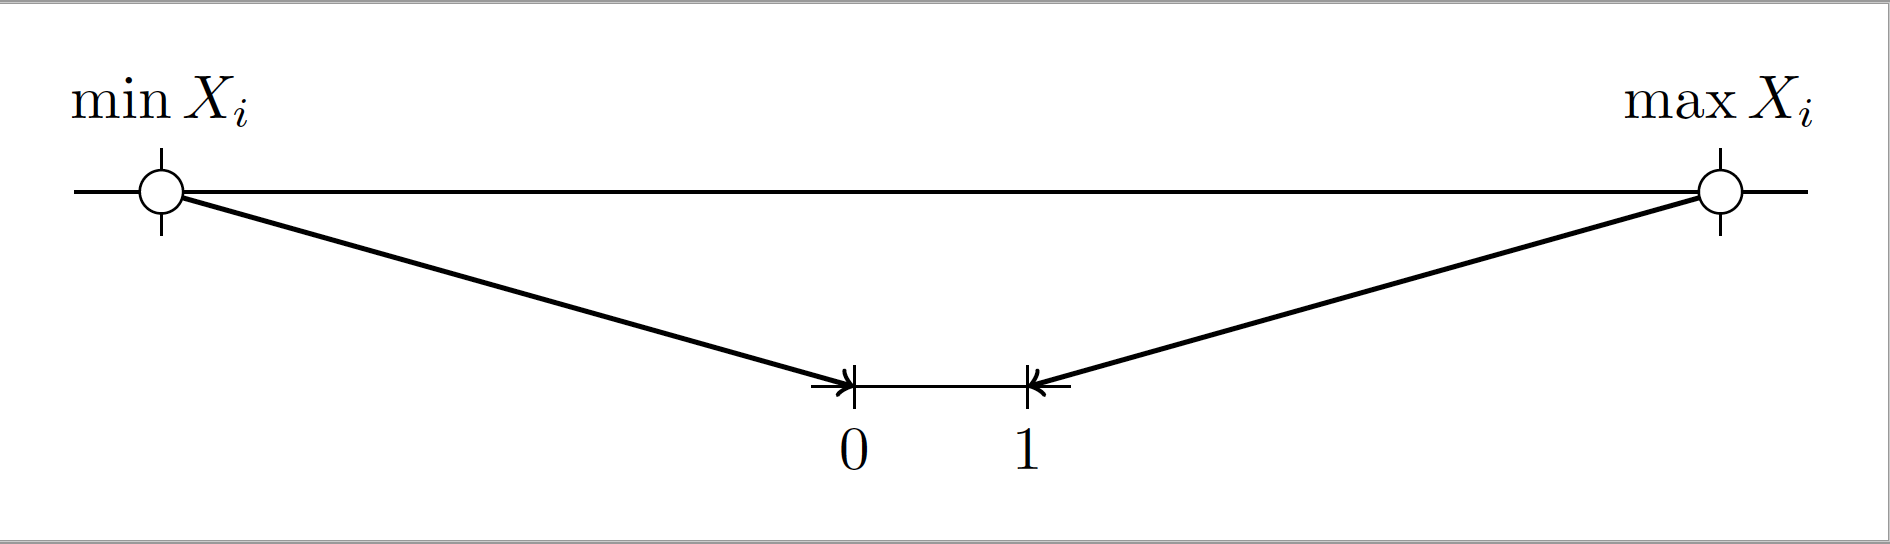
\includegraphics[scale=0.35]{../../Figures/fig_minmaxmap.png}
\end{figure}	
	
\end{frame}
\begin{frame}{Feature Standardization}
	If we have the variable $X$ we can use the transformation 
	\begin{equation*}
		\tilde{X}= \frac{ X - \mu}{\sigma},
	\end{equation*}
where $\mu=E(X)$ and $\sigma=\sigma(X)$.

{\bf Note.} The standardization relies on estimates of the mean and standard deviation.

\end{frame}
\begin{frame}{Cross validation}
	{\Large \bf Important Note}
	In this part, we will assume that we have access to the test dataset. 
	
	Roughly speaking, we will consider methods that estimate the {\bf test error rate} by {\it holding out} a subset of the training observations from the fitting process, and then applying the statistical learning method to those held out observations. 
	
\end{frame}

\begin{frame}{Leave-one-out cross-validation}
	LOOCV  involves splitting the set of observations into two parts. A single observation $(x_1,y_1)$ is used for the validation set, and the remaining observations $\{(x_2,y_2), \ldots, (x_n,y_n)\}$  make up for the training set. The statistical learning method is fir on the $n-1$ training observations and a prediction $\hat{y}_1$ is made fo the excluding observation. $MSE_1= (y_1-\hat{y}_1)^2$ provides an approximately unbiased estimate for the test error. 	
	We repeat this process for $(x_2,y_2)$ and so forth, then the LOOCV estimate for the test MSE is 
	\begin{equation*}
		CV_{(n)}=\frac{1}{n} \sum_{i=1}^n MSE_i
	\end{equation*}
\end{frame}

\begin{frame}{LOOCV idea}
	\begin{figure}
		\centering
		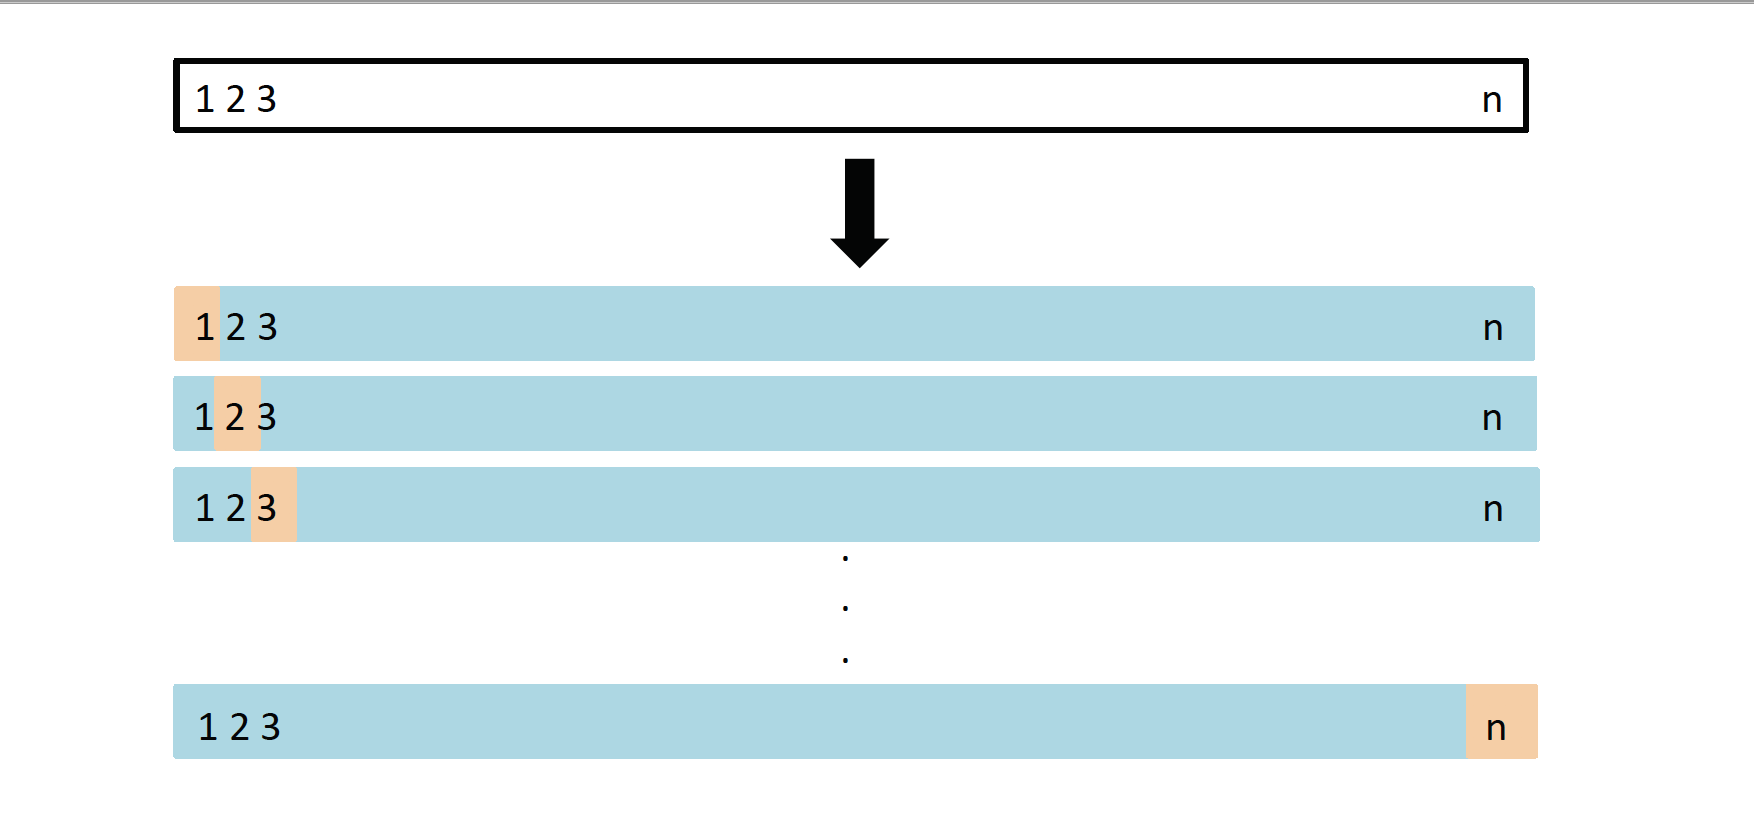
\includegraphics[scale=0.35]{../../Figures/fig_loocv.png}
	\end{figure}	
\end{frame}


\begin{frame}{$k$-fold Cross Validation}
	This approach involves randomly dividing the set of observations into $k$ groups, or folds, of approximately equal size. The first fold is treated as a validation set, and the method is fit on the remaining $k-1$ folds. The mean squared error $MSE_1$ is then computed on the observations in the held-out fold. This process is repeated $k$ times; each time, a different group of observations is treated as a validation set. This process results in $k$ estimates of the test error. The $k$-fold CV estimate is computed by averaging 
	\begin{equation*}
		CV_{(k)}=\frac 1k \sum_{i=1}^k MSE_i
	\end{equation*}
\end{frame}

\begin{frame}{$k$-fold CV idea}
	\begin{figure}
		\centering
		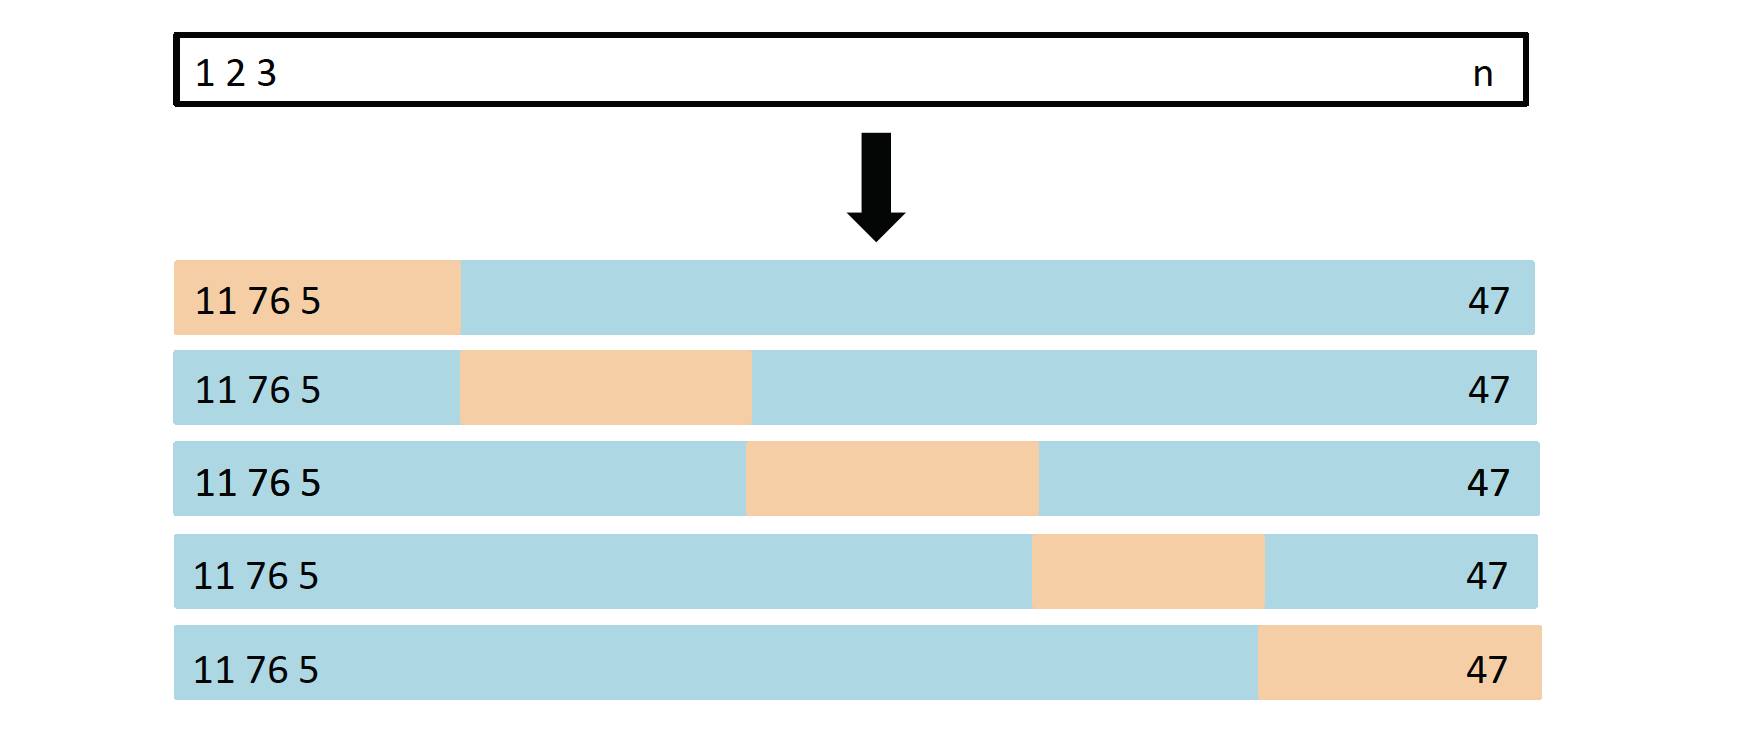
\includegraphics[scale=0.35]{../../Figures/fig_kfoldcv.png}
	\end{figure}	
\end{frame}

\begin{frame}{What have we learned?}
	\begin{itemize}
		\item Measures of performance commonly used in statistical models (RSE, RSS, RMSE).
		\item Common practices for preparing datasets for ML.
		\item Revisiting Expectation, Variance, Correlations and Variance-Covariance matrices.
		\item Best practices for data imputation.
		\item Data transformation.
		\item Cross validation as an estimate of test error. 
		
	\end{itemize}
\end{frame}


\begin{frame}{References}
	
\nocite{*}	
Materials and some of the pictures are from \citep{James2015}.
    \printbibliography 




I have used some of the graphs by hacking TiKz code from StakExchange and other old tricks of \TeX
\end{frame}		
\end{document}
%